\begin{technical}
    {\Large\textbf{Mathematical Foundations of the Banach—Tarski Paradox}}
    
    \textbf{Overview.}  
    The Banach-Tarski paradox states that a solid ball in \(\mathbb{R}^3\) can be partitioned into finitely many disjoint subsets and rearranged - using only rigid motions - into two identical copies of the original. The result depends on the Axiom of Choice, the existence of a free subgroup of \(\mathrm{SO}(3)\), and the absence of a finitely additive rotation-invariant measure on all subsets of the sphere.

    \textbf{Construction Outline.}
    \begin{itemize}[leftmargin=*]
        \item \textbf{Group-Theoretic Basis.}  
        The free group \(F_2 = \langle a, b \rangle\) is equidecomposable with two disjoint copies of itself under left multiplication. This violates the property of amenability, which forbids such duplications.

        \item \textbf{Geometric Embedding.}  
        Rotations \(S\) and \(T\) in \(\mathrm{SO}(3)\), each by angle \(\theta = \arccos(1/3)\) around orthogonal axes, generate a subgroup isomorphic to \(F_2\). No nontrivial reduced word in these rotations fixes any point off the axes.

        \item \textbf{Removing Fixed Points.}  
        The set \(D\) of all points fixed by nontrivial group elements is countable. One can remove \(D\) from the sphere by applying a suitable rotation to each of its images.

        \item \textbf{Orbit Decomposition.}  
        The action of \(F_2\) on \(S^2 \setminus D\) partitions it into orbits. The Axiom of Choice selects one representative per orbit to form a set \(M\). Then \(S^2 \setminus D = \bigsqcup_{g \in F_2} gM\).

        \item \textbf{Duplication via Equidecomposition.}  
        Since \(F_2 = A \sqcup B\) with \(A \cong F_2\) and \(B \cong F_2\), define bijections \(\phi_i : F_i \to F_2\), and extend them to \(S^2 \setminus D\) via \(x = gm \mapsto \phi_i(g)m\). This yields two disjoint subsets each equidecomposable with the whole.

        \item \textbf{Lifting to the Ball.}  
        The unit ball is viewed as concentric spherical shells. The paradoxical decomposition is applied to each shell simultaneously. The center is treated separately.
    \end{itemize}
    
    \columnbreak

    \textbf{Amenability and Non-Amenability.}  
    A group is amenable if there exists a finitely additive, invariant probability measure on all its subsets. Free groups on two or more generators are non-amenable: they admit no such measure. This failure is what allows equidecomposition of a set with two disjoint isometric copies of itself. The Banach-Tarski paradox is a geometric manifestation of non-amenability.

    \textbf{Cayley Graph Interpretation.}  
    The Cayley graph of \(F_2\) is a 4-regular tree. Each branch corresponds to a left coset, and the entire group acts by translation. It is somewhat easy to see that a careful merger of two opposite branches of the tree will result in a tree with the same structure as the original full tree, in a fractal way.

    \textbf{Rotations Generating the Free Group.}  
    Define $R = \frac{1}{3}\begin{bmatrix} 1 & -2\sqrt{2} \\ 2\sqrt{2} & 1 \end{bmatrix}$. Then:
    \[
    S = \begin{bmatrix} R & 0 \\ 0 & 1 \end{bmatrix}, \quad
    T = \begin{bmatrix} 1 & 0 \\ 0 & R \end{bmatrix}
    \]
    Any reduced word \(W\) in \(S\), \(T\), and their inverses maps \((1,0,0)\) to a vector of the form \(\left( \frac{a}{3^n}, \frac{\sqrt{b}}{3^n}, \frac{c}{3^n} \right)\), with \(b > 0\), confirming that the group acts freely on the orbit of \((1,0,0)\).

    \begin{center}
    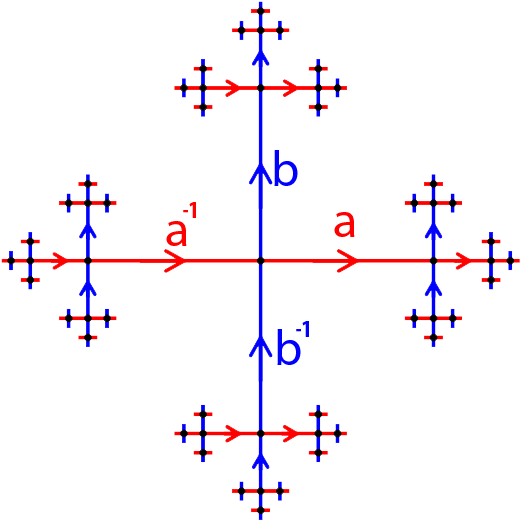
\includegraphics[width=0.4\textwidth]{01_BanachTarskiParadox/F2_Cayley_Graph_tp.png}

    \vspace{0.5em}
    \small
    \textbf{Figure:} Cayley graph of \(F_2\), visualized as a tree with no cycles and uniform branching.
    \end{center}

    \vspace{0.5em}
    \noindent\textbf{References} \\
    Banach, S. \& Tarski, A. (1924). \textit{Fund. Math.} \textbf{6}\\
    Wu, A. (2008). \textit{The Banach--Tarski Paradox}.
\end{technical}